\documentclass{../../ktane-mod}
\RequirePackage{enumitem}

\setlength{\parindent}{0pt}
\setlength{\parskip}{10pt}

\begin{document}
  \section*{Needy Modules}
  \rhead{Needy Modules}

  \vspace{0.4cm}
  \InsertBoxR{0}{
    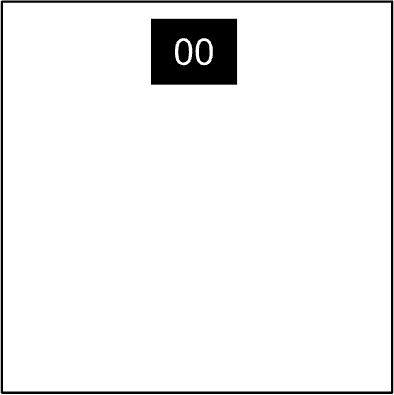
\includegraphics[height=3.5cm]{needy}
  }

  Needy modules cannot be disarmed, but pose a recurrent hazard.

  Needy modules can be identified as a module with a small 2-digit timer in the top center.
  Interacting with the bomb may cause them to become activated.
  Once activated, these needy modules must be tended to regularly before their timer expires in order to prevent a strike.

  Stay observant: needy modules may reactivate at any time.

  \vspace{2cm}

  \begin{needymodule}{
  moduleName=Capacitor Discharge,
  imageResource=modules/capacitor_discharge.pdf
}
{
  I'm going to guess that this is just meant to occupy your attention, because otherwise this is some shoddy electronics work.
}
  \begin{bulletlist}
    \bulletitem{Discharge the capacitor before it overloads by holding down the lever.}
  \end{bulletlist}

\end{needymodule}


  \begin{needymodule}{
  moduleName=Knobs,
  imageResource=modules/knobs.pdf
}
{
  Needlessly complicated and endlessly needy.
  Imagine if such expertise were used to make something other than diabolical puzzles.
}
  \begin{bulletlist}
    \bulletitem{The knob can be turned to one of four different positions.}
    \bulletitem{The knob must be in the correct position when this module's timer hits zero.}
    \bulletitem{The correct position can be determined by looking at the left half of the LEDs on the module.
      The six LEDs on the right are not relevant for solving this module.}
    \bulletitem{Knob positions are relative to the "UP" label, which may be rotated differently every time the module activates.}
  \end{bulletlist}

\textheading{The left six LEDs:}
  \begin{enumerate}[label=\alph{enumi}.]
    \item 0 or 1 LEDs lit -- Left
    \item 3 LEDs lit -- Down
    \item 4 LEDs lit -- Up
    \item 5 LEDs lit in "U"-Shape -- Right\\
    \vspace{0.2cm}
    \begin{tabular}{|c|c|c|}
    \hline
    X & & X \\
    \hline
    X & X & X \\
    \hline
    \end{tabular} \quad X marks a lit LED\@.
    \item Otherwise -- Down
  \end{enumerate}

\end{needymodule}


  \clearpage
  \begin{needymodule}{
  moduleName=Venting Gas,
  imageResource=modules/venting_gas_img.pdf
}
{
  Computer hacking is hard work!
  Well, it usually is.
  This job could probably be performed by a simple drinking bird pressing the same key over and over again.
}
  \begin{bulletlist}
    \bulletitem{Respond to the computer prompts by pressing "Y" for "Yes" or "N" for "No".}
  \end{bulletlist}

\end{needymodule}


\cleardoublepage
\end{document}
